%\VignetteIndexEntry{DLM}
%\VignettePackage{MARSS}
\documentclass[10pt]{article}

%\input{tex/mathdefs}
\usepackage{amsmath} % the standard math package
\usepackage[small, bf]{caption} % for nicer caption options
\setlength{\captionmargin}{24pt}
\usepackage{enumerate} % for nicer list options
%%%% bold maths symbol system:
\def\AA{\mbox{$\mathbf A$}}
\def\aa{\mbox{$\mathbf a$}}
\def\BB{\mbox{$\mathbf B$}}
\def\bb{\mbox{$\mathbf b$}}
\def\CC{\mbox{$\mathbf C$}}
\def\cc{\mbox{$\mathbf c$}}
\def\DD{\mbox{$\mathbf D$}}
\def\dd{\mbox{$\mathbf d$}}
\def\EE{\mbox{$\mathbf E$}}
\def\ee{\mbox{$\mathbf e$}}
\def\FF{\mbox{$\mathbf F$}}
\def\ff{\mbox{$\mathbf f$}}
\def\gg{\mbox{$\mathbf g$}}
\def\GG{\mbox{$\mathbf G$}}
\def\HH{\mbox{$\mathbf H$}}
\def\II{\mbox{$\mathbf I$}}
\def\LL{\mbox{$\mathbf L$}}
\def\MM{\mbox{$\mathbf M$}}
\def\mm{\mbox{$\mathbf m$}}
\def\OO{\mbox{$\mathbf O$}}
\def\PP{\mbox{$\mathbf P$}}
\def\pp{\mbox{$\mathbf p$}}
\def\QQ{\mbox{$\mathbf Q$}}
\def\qq{\mbox{$\mathbf q$}}
\def\RR{\mbox{$\mathbf R$}}
\def\rr{\mbox{$\mathbf r$}}
\def\UU{\mbox{$\mathbf U$}}
\def\uu{\mbox{$\mathbf u$}}
\def\VV{\mbox{$\mathbf V$}}
\def\vv{\mbox{$\mathbf v$}}
\def\WW{\mbox{$\mathbf W$}}
\def\ww{\mbox{$\mathbf w$}}
\def\XX{\mbox{$\mathbf X$}}
\def\xx{\mbox{$\mathbf x$}}
\def\YY{\mbox{$\mathbf Y$}}
\def\yy{\mbox{$\mathbf y$}}
\def\ZZ{\mbox{$\mathbf Z$}}
\def\zz{\mbox{$\mathbf z$}}
\def\et{\mbox{\boldmath $\eta$}}
\def\ep{\mbox{\boldmath $\epsilon$}}
\def\pipi{\mbox{\boldmath $\pi$}}
\def\uupsilon{\pmb{\upsilon}}
\def\llambda{\pmb{\lambda}}
\def\bbeta{\pmb{\beta}}
\def\aalpha{\pmb{\alpha}}
\def\zzeta{\pmb{\zeta}}
\def\etaeta{\mbox{\boldmath $\eta$}}
\def\xixi{\mbox{\boldmath $\xi$}}
\def\ttheta{\mbox{\boldmath $\theta$}}
\def\PI{\mbox{\boldmath $\mathrm{\Pi}$}}
\def\LAM{\mbox{\boldmath $\mathrm{\Lambda}$}}
\def\GAM{\mbox{\boldmath $\mathrm{\Gamma}$}}
\def\SI{\mbox{\boldmath $\mathrm{\Sigma}$}}
\def\THETA{\mbox{\boldmath $\mathrm{\Theta}$}}
\def\PH{\mbox{\boldmath $\mathrm{\Phi}$}}
\def\zer{\mbox{\boldmath $0$}}
\def\vec{\,\textup{\textrm{vec}}}
\def\var{\,\textup{\textrm{Var}}}
\def\cov{\,\textup{\textrm{cov}}}
\def\diag{\,\textup{\textrm{diag}}}
\def\MVN{\,\textup{\textrm{MVN}}}
\def\AIC{\,\textup{\textrm{AIC}}}
\def\E{\,\textup{\textrm{E}}}
\def\Lik{\,\textup{\textrm{L}}}
\def\N{\,\textup{\textrm{N}}}
\def\R{R}


%-----------------------------------------------


\usepackage{Sweave}
\begin{document}
\Sconcordance{concordance:DLM_lab_5.tex:DLM_lab_5.Rnw:%
1 78 1 1 7 2 1 1 0 72 1 1 3 2 0 1 2 1 0 1 2 1 0 1 2 4 0 1 2 1 1 1 3 2 0 %
1 2 1 0 1 2 4 0 1 2 3 1 1 6 1 2 5 1 1 3 2 0 3 1 3 0 1 2 1 1 1 3 2 0 4 1 %
3 0 1 2 1 1 1 3 2 0 1 2 4 0 1 2 1 3 27 0 1 2 8 1 1 16 1 2 29 1 1 3 2 0 %
1 2 1 0 1 2 1 0 1 3 5 0 1 2 1 1 1 3 2 0 1 2 1 0 1 2 1 0 1 4 6 0 1 2 6 1 %
1 10 1 2 10 1 1 14 1 2 15 1 1 3 5 0 1 2 1 1 1 3 2 0 1 2 4 0 1 2 4 1 1 8 %
1 6 5 1 1 3 8 0 1 2 2 1 1 3 5 0 1 2 4 1 1 7 1 2 64 1 1 9 8 0 1 3 13 0 1 %
2 33 1 1 4}

%\SweaveOpts{keep.source=TRUE, prefix.string=./figures/CSX-, eps=FALSE, split=FALSE}
%\chapter{Case Study X: Dynamic linear models (DLMs)}
%\label{chap:DLM}
%\chaptermark{Dynamic linear models}
%\part{Case Study X: Dynamic linear models (DLMs)}
\section{Overview of dynamic linear models}
\index{MARSS model!DLM example}Here we will use MARSS to analyze dynamic linear models (DLMs), wherein the parameters in a regression model are treated as time-varying. DLMs are used commonly in econometrics, but have received less attention in the ecological literature (c.f., Lamon et al. 1998, Scheuerell and Williams 2005). Our treatment of DLMs is rather cursory---we direct the reader to excellent textbooks by Pole et al. (1994) and Petris et al. (2009) for more in-depth treatments of DLMs. The former focuses on Bayesian estimation whereas the latter addresses both likelihood-based and Bayesian estimation methods.

We begin our description of DLMs with a $static$ regression model, wherein the $i^{th}$ observation is a linear function of an intercept, predictor variable(s), and a random error term. For example, if we had one predictor variable ($F$), we could write the model as
\begin{equation}\label{eqn:lm}
y_i = \alpha + \beta F_i + v_i,
\end{equation}
where the $\alpha$ is the intercept, $\beta$ is the regression slope, $F_i$ is the predictor variable matched to the $i^{th}$ observation ($y_i$), and $v_i \sim \N(0,r)$. It is important to note here that there is no implicit ordering of the index $i$. That is, we could shuffle any/all of the $(y_i, F_i)$ pairs in our dataset with no effect on our ability to estimate the model parameters. We can write the model in Eqn \ref{eqn:lm} using vector notation, such that
\begin{align}\label{eqn:lmVec}
y_i &= \begin{pmatrix}1&F_i\end{pmatrix} \times
\begin{pmatrix}\alpha\\ \beta\end{pmatrix} + v_i \nonumber\\
&= \FF_i^{\top}\ttheta + v_i,
\end{align}
and $\FF_i^{\top} = (1,F_i)$ and $\ttheta = (\alpha,\beta)^{\top}$.

In a DLM, however, the regression parameters are $dynamic$ in that they ``evolve'' over time. For a single observation at time $t$, we can write
\begin{equation}\label{eqn:dlm1}
y_t = \FF_{t}^{\top}\ttheta_t + v_t,
\end{equation}
where $\FF_t$ is a column vector of regression variables at time $t$, $\ttheta_t$ is a column vector of regression parameters at time $t$ and $v_{t}\sim\N(0,r)$. This formulation presents two features that distinguish it from Eqn \ref{eqn:lmVec}. First, the observed data are explicitly time ordered (i.e., $\yy=\lbrace{y_1,y_2,y_3,...,y_T}\rbrace$), which means we expect them to contain implicit information. Second, the relationship between the observed datum and the predictor variables are unique at every time $t$ (i.e., $\ttheta=\lbrace{\ttheta_1,\ttheta_2,\ttheta_3,...,\ttheta_T}\rbrace$).

However, closer examination of Eqn \ref{eqn:dlm1} reveals an apparent complication for parameter estimation. With only one datum at each time step $t$, we could, at best, estimate only one regression parameter, and even then, the 1:1 correspondence between data and parameters would preclude any estimation of parameter uncertainty. To address this shortcoming, we return to the time ordering of model parameters. Rather than assume the regression parameters are independent from one time step to another, we instead model them as an autoregressive process where
\begin{equation}\label{eqn:dlm2}
\ttheta_t = \GG_t\ttheta_{t-1} + \ww_t,
\end{equation}
$\GG_t$ is the parameter ``evolution'' matrix, and $\ww_t$ is a vector of process errors, such that $\ww_t\sim\MVN(\mathbf{0},\QQ)$. The elements of $\GG_t$ may be known and fixed \textit{a priori}, or unknown and estimated from the data. Although we allow for $\GG_t$ to be time-varying, we will typically assume that it is time invariant.

The idea is that the evolution matrix $\GG_t$ deterministically maps the parameter space from one time step to the next, so the parameters at time $t$ are temporally related to those before and after. However, the process is corrupted by stochastic error, which amounts to a degradation of information over time. If the diagonal elements of $\QQ$ are relatively large, then the parameters can vary widely from $t$ to $t+1$. If $\QQ\ = \mathbf{0}$, then $\ttheta_1=\ttheta_2=\ttheta_T$ and we are back to the static model in Eqn \ref{eqn:lm}.


%------------------------------------
\section{Example of a univariate DLM}
%------------------------------------
Let's consider an example from the literature. Scheuerell \& Williams (2005) used a DLM to examine the relationship between marine survival of Chinook salmon and an index of ocean upwelling strength along the west coast of the USA. Upwelling brings cool, nutrient-rich waters from the deep ocean to shallower coastal areas. Scheuerell \& Williams hypothesized that stronger upwelling in April should create better growing conditions for phytoplankton, which would then translate into more zooplankton. In turn, juvenile salmon (``smolts'') entering the ocean in May and June should find better foraging opportunities. Thus, for smolts entering the ocean in year $t$,
\begin{equation}\label{eqn:dlmSW1}
survival_t = \alpha_t + \beta_t F_t + v_t \text{ with } v_{t}\sim\N(0,r),
\end{equation}
and $F_t$ is the coastal upwelling index (cubic meters of seawater per second per 100 m of coastline) for the month of April in year $t$. 

Both the intercept and slope are time varying, so
% full univariate DLM as MARSS
\begin{align}\label{eqn:dlmSW2}
\alpha_t &= \alpha_{t-1} + w_t^{(\alpha)} \text{ with } w_t^{(\alpha)} \sim \N(0,q_{\alpha}); \text{ and}\\
\beta_t &= \beta_{t-1} + w_t^{(\beta)} \text{ with } w_t^{(\beta)} \sim \N(0,q_{\beta}).
\end{align}
If we define $\ttheta_t = (\alpha_t,\beta_t)^{\top}$, $\GG_t = \II \; \forall \; t$, $\ww_t = (w_t^{(1)},w_t^{(2)})^{\top}$, and $\QQ = \diag(q_1,q_2)$, we get Eqn \ref{eqn:dlm2}. If we define $y_t = survival_t$ and $\FF_t = (1,F_t)^{\top}$, we can write out the full univariate DLM as a state-space model with the following form:
\begin{equation}\label{eqn:dlmSW3}
\begin{gathered}
\ttheta_t = \GG_t\ttheta_{t-1} + \ww_t \text{ with } \ww_t \sim \MVN(\mathbf{0},\QQ);\\
y_t = \FF_t^{\top}\ttheta_t + v_t \text{ with } v_t\sim\N(0,r);\\
\ttheta_0 \sim \MVN(\pipi_0,\LAM_0).
\end{gathered}
\end{equation}
Eqn \ref{eqn:dlmSW3} is, not surprisingly, equivalent to our standard MARSS model: 
\begin{equation}\label{eqn:MARSSdlm}
\begin{gathered}
\xx_t = \BB_t\xx_{t-1} + \uu_t + \CC_t\cc_t + \ww_t \text{ with } \ww_t \sim \MVN(0,\QQ_t);\\
\yy_t = \ZZ_t\xx_t + \aa_t + \DD_t\dd_t + \vv_t \text{ with } \vv_t \sim \MVN(0,\RR_t);\\
\xx_0 \sim \MVN(\pipi,\LAM);
\end{gathered}
\end{equation}
where $\xx_t = \ttheta_t$, $\BB_t = \GG_t$, $\uu_t = \CC_t = \cc_t = \zer$, $\yy_t = y_t$ (i.e., $\yy_t$ is 1 $\mathsf{x}$ 1), $\ZZ_t = \FF_t^{\top}$, $\aa_t = \DD_t = \dd_t = \zer$, and $\RR_t = r$ (i.e., $\RR_t$ is 1 $\mathsf{x}$ 1).
%------------------------------------------------
\subsection{Fitting a univariate DLM with MARSS}
%------------------------------------------------
Now let's go ahead and analyze the DLM specified in Eqns \ref{eqn:dlmSW1}--\ref{eqn:dlmSW3}. We begin by getting the data set, which has 3 columns for 1) the year the salmon smolts migrated to the ocean ($year$), 2) logit-transformed survival\footnote{Survival in the original context was defined as the proportion of juveniles that survive to adulthood. Thus, we use the logit function, defined as $logit(p)=log_e(p/[1-p])$, to map survival from the open interval (0,1) onto the interval $(-\infty,\infty)$, which allows us to meet our assumption of normally distributed observation errors.} ($logit.s$), and 3) the coastal upwelling index for April ($CUI.apr$). There are 42 years of data (1964--2005).
\begin{Schunk}
\begin{Sinput}
 ## load the data
 data(SalmonSurvCUI)
 ## get time indices
 years = SalmonSurvCUI[,1]
 ## number of years of data
 TT = length(years)
 ## get response data: logit(survival)
 dat = matrix(SalmonSurvCUI[,2],nrow=1)
\end{Sinput}
\end{Schunk}

As we have seen in other case studies, standardizing our covariate(s) to have zero-mean and unit-variance can be helpful in model fitting and interpretation. In this case, it's a good idea because the variance of $CUI.apr$ is orders of magnitude greater than $survival$.
\begin{Schunk}
\begin{Sinput}
 ## get regressor variable
 CUI = SalmonSurvCUI[,3]
 ## z-score the CUI
 CUI.z = matrix((CUI - mean(CUI))/sqrt(var(CUI)), nrow=1)
 ## number of regr params (slope + intercept)
 m = dim(CUI.z)[1] + 1
\end{Sinput}
\end{Schunk}
Plots of logit-transformed survival and the $z$-scored April upwelling index are shown in Figure \ref{fig:CSX.fig1}.

\begin{figure}[htp]
\begin{center}
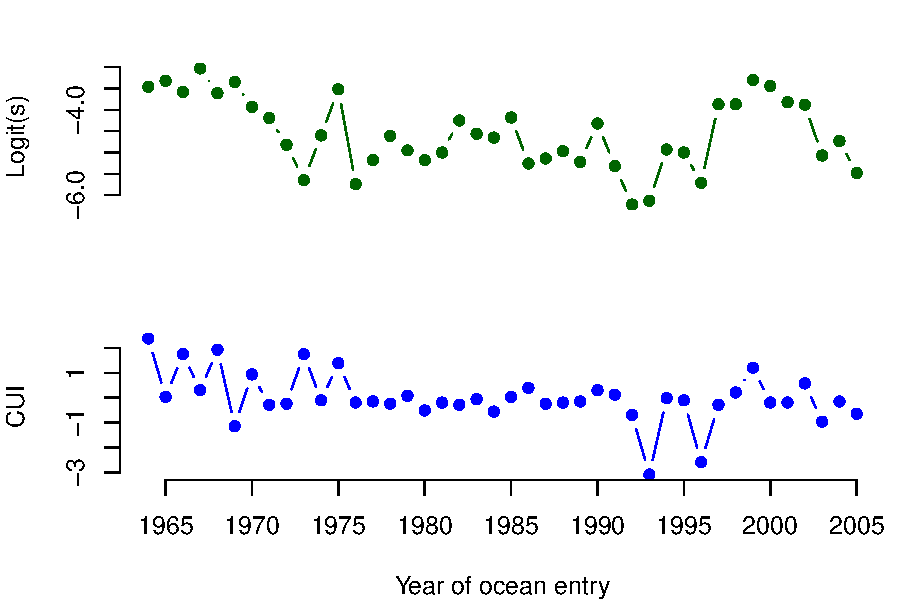
\includegraphics{DLM_lab_5-plotdata}
\end{center}
\caption{Time series of logit-transformed marine survival estimates for Snake River spring/summer Chinook salmon (top) and \textit{z}-scores of the coastal upwelling index at 45N 125W (bottom). The \textit{x}-axis indicates the year that the salmon smolts entered the ocean.}
\label{fig:CSX.fig1}
\end{figure}

Next, we need to set up the appropriate matrices and vectors for MARSS. Let's begin with those for the process equation because they are straightforward.
\begin{Schunk}
\begin{Sinput}
 ## for process eqn
 B = diag(m)                     ## 2x2; Identity
 U = matrix(0,nrow=m,ncol=1)     ## 2x1; both elements = 0
 Q = matrix(list(0),m,m)         ## 2x2; all 0 for now
 diag(Q) = c("q.alpha","q.beta") ## 2x2; diag = (q1,q2)
\end{Sinput}
\end{Schunk}

Defining the correct form for the observation model is a little more tricky, however, because of how we model the effect(s) of explanatory variables. In a DLM, we need to use $\ZZ_t$ (instead of $\dd_t$) as the matrix of known regressors/drivers that affect $\yy_t$, and $\xx_t$ (instead of $\DD_t$) as the regression parameters. Therefore, we need to set $\ZZ_t$ equal to an $n$ $\mathsf{x}$ $m$ $\mathsf{x}$ $T$ array, where $n$ is the number of response variables (= 1; $y_t$ is univariate), $m$ is the number of regression parameters (= intercept + slope = 2), and $T$ is the length of the time series (= 42). 
\begin{Schunk}
\begin{Sinput}
 ## for observation eqn
 Z = array(NA, c(1,m,TT))   ## NxMxT; empty for now
 Z[1,1,] = rep(1,TT)        ## Nx1; 1's for intercept
 Z[1,2,] = CUI.z            ## Nx1; regr variable
 A = matrix(0)              ## 1x1; scalar = 0
 R = matrix("r")            ## 1x1; scalar = r
\end{Sinput}
\end{Schunk}

Lastly, we need to define our lists of initial starting values and model matrices/vectors. 
\begin{Schunk}
\begin{Sinput}
 ## only need starting values for regr parameters
 inits.list = list(x0=matrix(c(0, 0), nrow=m))
 ## list of model matrices & vectors
 mod.list = list(B=B, U=U, Q=Q, Z=Z, A=A, R=R)
\end{Sinput}
\end{Schunk}
And now we can fit our DLM with MARSS.
\begin{Schunk}
\begin{Sinput}
 ## fit univariate DLM
 dlm1 = MARSS(dat, inits=inits.list, model=mod.list)
\end{Sinput}
\begin{Soutput}
Success! abstol and log-log tests passed at 115 iterations.
Alert: conv.test.slope.tol is 0.5.
Test with smaller values (<0.1) to ensure convergence.

MARSS fit is
Estimation method: kem 
Convergence test: conv.test.slope.tol = 0.5, abstol = 0.001
Estimation converged in 115 iterations. 
Log-likelihood: -40.03813 
AIC: 90.07627   AICc: 91.74293   
 
          Estimate
R.r        0.15708
Q.q.alpha  0.11264
Q.q.beta   0.00564
x0.X1     -3.34023
x0.X2     -0.05388

Standard errors have not been calculated. 
Use MARSSparamCIs to compute CIs and bias estimates.
\end{Soutput}
\end{Schunk}

Notice that the MARSS output does not list any estimates of the regression parameters themselves. Why not? Remember that in a DLM the matrix of states $(\xx)$ contains the estimates of the regression parameters $(\ttheta)$. Therefore, we need to look in \verb@dlm1$states@ for the MLEs of the regression parameters, and in \verb@dlm1$states.se@ for their standard errors.

Time series of the estimated intercept and slope are shown in Figure \ref{fig:CSX.fig2}. It appears as though the intercept is much more dynamic than the slope, as indicated by a much larger estimate of process variance for the former (\verb@Q.q1@). In fact, although the effect of April upwelling appears to be increasing over time, it doesn't really become important as an explanatory variable until about 1990 when the approximate 95\% confidence interval for the slope no longer overlaps zero.
%----------------------------
% plot regression parameters
%----------------------------
\begin{figure}[htp]
\begin{center}
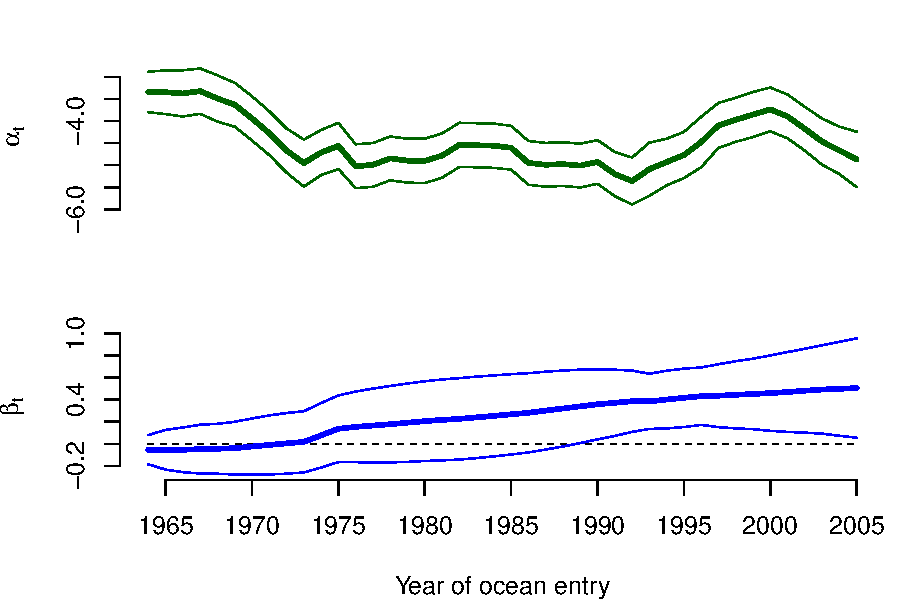
\includegraphics{DLM_lab_5-plotdlm1}
\end{center}
\caption{Time series of estimated mean states (thick lines) for the intercept (top) and slope (bottom) parameters from the univariate DLM specified by Eqns \ref{eqn:dlmSW1}--\ref{eqn:dlmSW3}. Thin lines denote the mean $\pm$ 2 standard deviations.}
\label{fig:CSX.fig2}
\end{figure}
%----------------------------------------------
\section{Forecasting with a univariate DLM}
%----------------------------------------------
Scheuerell \& Williams (2005) were interested in how well upwelling could be used to actually \textit{forecast} expected survival of salmon, so let's look at how well our model does in that context. To do so, we need the predictive distributions for the regression parameters and observation.

Beginning with our definition for the distribution of the parameters at time $t=0$, $\ttheta_0 \sim \MVN(\pipi_0,\LAM_0)$ in Eqn \ref{eqn:dlmSW3}, we write
\begin{equation}\label{eqn:dlmFore1}
\ttheta_{t-1}|y_{1:t-1} \sim \MVN(\pipi_{t-1},\LAM_{t-1})
\end{equation}
to indicate the distribution of $\ttheta$ at time $t-1$ conditioned on the observed data through time $t-1$ (i.e., $y_{1:t-1}$). Then, we can write the one-step ahead predictive distribution for $\ttheta_t$ given $y_{1:t-1}$ as
\begin{align}\label{eqn:dlmFore2}
\ttheta_{t}|y_{1:t-1} &\sim \MVN(\et_{t},\PH_{t}), \text{ where} \nonumber\\
\et_{t} &= \GG_t\pipi_{t-1}, \text{ and}\\
\PH_{t} &= \GG_t\LAM_{t-1}\GG_t^{\top} + \QQ \nonumber.
\end{align}
Consequently, the one-step ahead predictive distribution for the observation at time $t$ given $y_{1:t-1}$ is
\begin{align}\label{eqn:dlmFore3}
y_{t}|y_{1:t-1} &\sim \N(\zeta_{t},\Psi_{t}), \text{ where} \nonumber\\
\zeta_{t} &= \FF_t\et_{t}, \text{ and}\\
\Psi_{t} &= \FF_t\Phi_{t}\FF_t^{\top} + \RR \nonumber.
\end{align}

%----------------------------------------------
\subsection{Forecasting a univariate DLM with MARSS}
%----------------------------------------------
Working from Eqn \ref{eqn:dlmFore3}, we can now use MARSS to compute the expected value of the forecast at time $t$ $(\E [y_t|y_{1:t-1}] = \zeta_t)$, and its variance $(\var [y_t|y_{1:t-1}] = \Psi_t)$. For the expectation, we need $\FF_t\et_t$. Recall that $\FF_t$ is our $1 \times m$ matrix of explanatory variables at time $t$ ($\FF_t$ is called $\ZZ_t$ in MARSS notation). The one-step ahead forecasts of the parameters at time $t$ $(\et_t)$ are calculated as part of the Kalman filter algorithm---they are termed $\tilde{x}_t^{t-1}$ in MARSS notation and stored as \verb@'xtt1'@ in the list produced by the \verb@MARSSkfss()@ function.
\begin{Schunk}
\begin{Sinput}
 ## get list of Kalman filter output
 kf.out = MARSSkfss(dlm1)
 ## forecasts of regr parameters; 2xT matrix
 eta = kf.out$xtt1
 ## ts of E(forecasts)
 fore.mean = vector()
 for(t in 1:TT) {
   fore.mean[t] = Z[,,t] %*% eta[,t,drop=F]
 }
\end{Sinput}
\end{Schunk}

For the variance of the forecasts, we need $\FF_t\Phi_{t}\FF_t^{\top} + \RR$. As with the mean, $\FF_t \equiv \ZZ_t$. The variances of the one-step ahead forecasts of the parameters at time $t$ $(\Phi_t)$ are also calculated as part of the Kalman filter algorithm---they are stored as \verb@'Vtt1'@ in the list produced by the \verb@MARSSkfss()@ function. Lastly, the observation variance $\RR$ is part of the standard MARSS output.
\begin{Schunk}
\begin{Sinput}
 ## variance of regr parameters; 1x2xT array
 Phi = kf.out$Vtt1
 ## obs variance; 1x1 matrix
 R.est = coef(dlm1, type="matrix")$R
 ## ts of Var(forecasts)
 fore.var = vector()
 for(t in 1:TT) {
   tZ = matrix(Z[,,t],m,1) ## transpose of Z
   fore.var[t] = Z[,,t] %*% Phi[,,t] %*% tZ + R.est
 }
\end{Sinput}
\end{Schunk}

Plots of the model mean forecasts with their estimated uncertainty are shown in Figure \ref{fig:CSX.fig3}. Nearly all of the observed values fell within the approximate prediction interval. Notice that we have a forecasted value for the first year of the time series (1964), which may seem at odds with our notion of forecasting at time $t$ based on data available only through time $t-1$. In this case, however, MARSS is actually estimating the states at $t=0$ ($\ttheta_0$), which allows us to compute a forecast for the first time point.
%-----------------------------
% forecast plot - logit space
%-----------------------------
\begin{figure}[htp]
\begin{center}
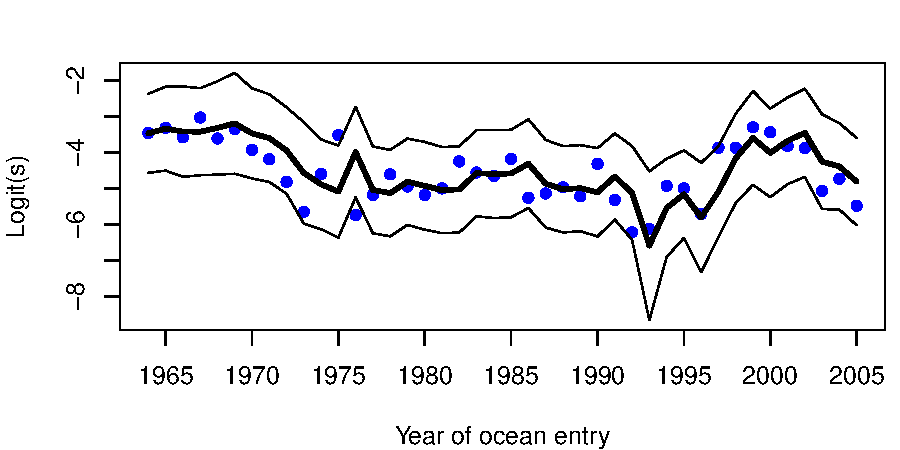
\includegraphics{DLM_lab_5-plotdlmForeLogit}
\end{center}
\caption{Time series of logit-transformed survival data (blue dots) and model mean forecasts (thick line). Thin lines denote the approximate 95\% prediction intervals.}
\label{fig:CSX.fig3}
\end{figure}

Although our model forecasts look reasonable in logit-space, it is worthwhile to examine how well they look when the survival data and forecasts are back-transformed onto the interval [0,1] (Figure \ref{fig:CSX.fig4}). In that case, the accuracy does not seem to be affected, but the precision appears much worse, especially during the early and late portions of the time series when survival is changing rapidly.
%------------------------------
% forecast plot - normal space
%------------------------------
\begin{figure}[htp]
\begin{center}
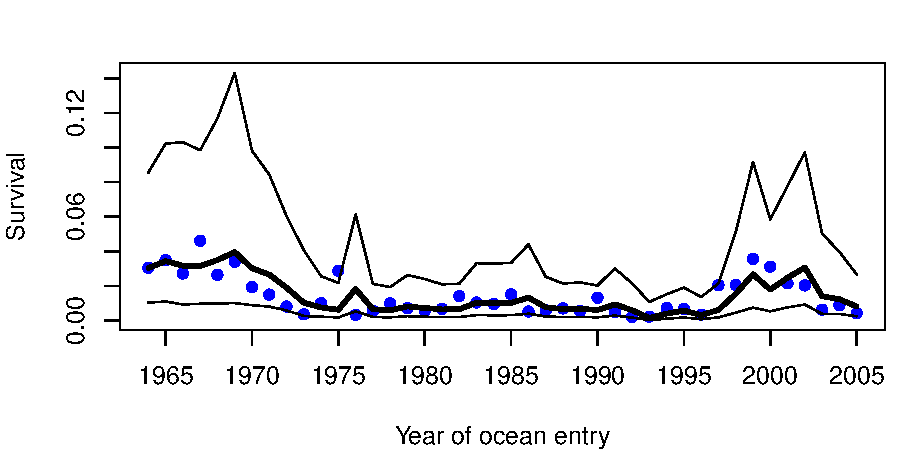
\includegraphics{DLM_lab_5-plotdlmForeRaw}
\end{center}
\caption{Time series of survival data (blue dots) and model mean forecasts (thick line). Thin lines denote the approximate 95\% prediction intervals.}
\label{fig:CSX.fig4}
\end{figure}
%-------------------------------------
\subsection{DLM forecast diagnostics}
%-------------------------------------
\begin{samepage}
As with other time series models, evaluation of a DLM should include some model diagnostics. In a forecasting context, we are often interested in the forecast errors, which are simply the observed data minus the forecasts $(e_t = y_t - \zeta_t)$. In particular, the following assumptions should hold true for $e_t$:
\begin{enumerate}[1)]
\item $e_t \sim \N(0,\sigma^2)$;
\item $\cov(e_t,e_{t-k}) = 0$.
\end{enumerate}
\end{samepage}

In the literature on state-space models, the set of $e_t$ are commonly referred to as ``innovations''. \verb@MARSS()@ calculates the innovations as part of the Kalman filter algorithm---they are stored as \verb@'Innov'@ in the list produced by the \verb@MARSSkfss()@ function.
\begin{Schunk}
\begin{Sinput}
 ## forecast errors
 innov = kf.out$Innov
\end{Sinput}
\end{Schunk}

Let's see if our innovations meet the model assumptions. Beginning with (1), we can use a Q-Q plot to see whether the innovations are normally distributed with a mean of zero. We'll use the \verb@qqnorm()@ function to plot the quantiles of the innovations on the $y$-axis versus the theoretical quantiles from a Normal distribution on the $x$-axis. If the 2 distributions are similar, the points should fall on the line defined by $y = x$.
\begin{Schunk}
\begin{Sinput}
 ## Q-Q plot of innovations
 qqnorm(t(innov), main="", pch=16, col="blue")
 ## add y=x line for easier interpretation
 qqline(t(innov))
\end{Sinput}
\end{Schunk}
%----------------------
% diagnostics plot: QQ
%----------------------
\begin{figure}[htp]
\begin{center}
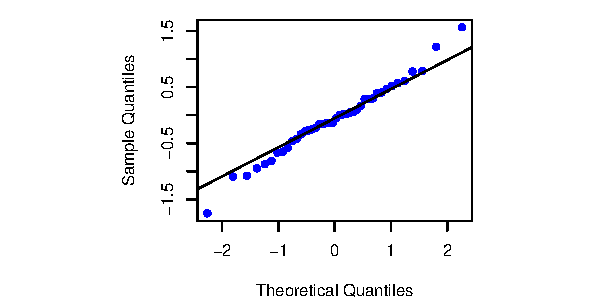
\includegraphics{DLM_lab_5-plotdlmQQ}
\end{center}
\caption{Q-Q plot of the forecast errors (innovations) for the DLM specified in Eqns \ref{eqn:dlmSW1}--\ref{eqn:dlmSW3}.}
\label{fig:CSX.fig5}
\end{figure}

The Q-Q plot (Figure \ref{fig:CSX.fig5}) indicates that the innovations appear to be more-or-less normally distributed (i.e., most points fall on the line). Furthermore, it looks like the mean of the innovations is about 0, but we should use a more reliable test than simple visual inspection. We can formally test whether the mean of the innovations is significantly different from 0 by using a one-sample $t$-test.  based on a null hypothesis of $\E(e_t)=0$. To do so, we will use the function \verb@t.test()@ and base our inference on a significance value of $\alpha = 0.05$.
\begin{Schunk}
\begin{Sinput}
 ## p-value for t-test of H0: E(innov) = 0
 t.test(t(innov), mu=0)$p.value
\end{Sinput}
\begin{Soutput}
[1] 0.4840901
\end{Soutput}
\end{Schunk}
The $p$-value $>>$ 0.05 so we cannot reject the null hypothesis that $\E(e_t)=0$.

Moving on to assumption (2), we can use the sample autocorrelation function (ACF) to examine whether the innovations covary with a time-lagged version of themselves. Using the \verb@acf()@ function, we can compute and plot the correlations of $e_t$ and $e_{t-k}$ for various values of $k$. Assumption (2) will be met if none of the correlation coefficients exceed the 95\% confidence intervals defined by $\pm \, z_{0.975} / \sqrt{n}$.
\begin{Schunk}
\begin{Sinput}
 ## plot ACF of innovations
 acf(t(innov), lag.max=10)
\end{Sinput}
\end{Schunk}
%-----------------------
% diagnostics plot: ACF
%-----------------------
\begin{figure}[htp]
\begin{center}
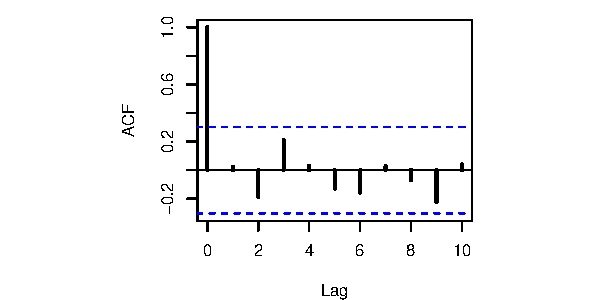
\includegraphics{DLM_lab_5-plotdlmACF}
\end{center}
\caption{Autocorrelation plot of the forecast errors (innovations) for the DLM specified in Eqns \ref{eqn:dlmSW1}--\ref{eqn:dlmSW3}. Horizontal blue lines define the upper and lower 95\% confidence intervals.}
\label{fig:CSX.fig6}
\end{figure}
The ACF plot (Figure \ref{fig:CSX.fig6}) shows no significant autocorrelation in the innovations at lags 1--10, so it looks like both of our model assumptions have indeed been met.


\newpage

%==========================
\section{Homework problems}
%==========================

For the homework this week we will use a DLM to examine some of the time-varying properties of the spawner-recruit relationship for Pacific salmon.  Much work has been done on this topic, particularly by Randall Peterman and his students and post-docs at Simon Fraser University.  To do so, researchers commonly use a Ricker model because of its relatively simple form, such that the number of recruits (offspring) born in year $t$ ($R_t$) from the number of spawners (parents) ($S_t$) is

\begin{equation}\label{eqn:baseRicker}
R_t = a S_t e^{-b S + v_t}.
\end{equation}


\noindent The parameter $a$ determines the maximum reproductive rate in the absence of any density-dependent effects (the slope of the curve at the origin), $b$ is the strength of density dependence, and $v_t \sim N(0,\sigma)$.  In practice, the model is typically log-transformed so as to make it linear with respect to the predictor variable $S_t$, such that

\begin{equation}\label{eqn:lnRicker}
\begin{aligned}
\text{log}(R_t) &= \text{log}(a) + \text{log}(S_t) -b S_t + v_t \\
\text{log}(R_t) - \text{log}(S_t) &= \text{log}(a) -b S_t + v_t \\
\text{log}(R_t/S_t) &= \text{log}(a) - b S_t + v_t.
\end{aligned}
\end{equation}


\noindent Substituting $y_t = \text{log}(R_t/S_t)$, $x_t = S_t$, and $\alpha = \text{log}(a)$ yields a simple linear regression model with intercept $\alpha$ and slope $b$.

Unfortunately, however, residuals from this simple model typically show high-autocorrelation due to common environmental conditions that affect overlaping generations.  Therefore, to correct for this and allow for an index of stock productivity that controls for any density-dependent effects, the model may be re-witten as

\begin{equation}\label{eqn:lnTVRicker}
\begin{aligned}
\text{log}(R_t/S_t) &= \alpha_t - b S_t + v_t, \\
\alpha_t &= \alpha_{t-1} + w_t,
\end{aligned}
\end{equation}

\noindent and $w_t \sim N(0,q)$.  By treating the brood-year specific productivity as a random walk, we allow it to vary, but in an autocorrelated manner so that consecutive years are not independent from one another.

More recently, interest has grown in using covariates ($e.g.$, sea-surface temperature) to explain the interannual variability in productivity.  In that case, we can can write the model as

\begin{equation}\label{eqn:lnCovRicker}
\text{log}(R_t/S_t) = \alpha + \delta_t X_t - b S_t + v_t.
\end{equation}

\noindent In this case we are estimating some base-level productivity ($\alpha$) plus the time-varying effect of some covariate $X_t$ ($\delta_t$). 


%--------------------------------
\subsection{Spawner-recruit data}
%--------------------------------

The data come from a large public database begun by Ransom Myers many years ago.  If you are interested, you can find lots of time series of spawning-stock, recruitment, and harvest for a variety of fishes around the globe.  Here is the website:\\

\verb@http://ram.biology.dal.ca/~myers/about_site.html@\\

For this exercise, we will use spawner-recruit data for sockeye salmon ($Oncorhynchus$ $nerka$) from the Kvichak River in SW Alaska that span the years 1952-1989.  In addition, we'll examine the potential effects of the Pacific Decadal Oscillation (PDO) during the salmon's first year in the ocean, which is widely believed to be a "bottleneck" to survival.

Here are the data:

\begin{Schunk}
\begin{Sinput}
 ## get S-R data; object is 'SRdata"
 ## file cols are:
 ## 1: brood yr (brood.yr)
 ## 2: number of spawners (Sp)
 ## 3: number of recruits (Rec)
 ## 4: PDO during first summer at sea (PDO.t2)
 ## 5: PDO during first winter at sea (PDO.t3)
 load("KvichakSockeye.RData")
 ## head of data file
 head(SRdata)
\end{Sinput}
\begin{Soutput}
  brood.yr   Sp   Rec PDO.t2 PDO.t3
1     1952 5970 17310  -0.61  -0.61
2     1953  320   520  -1.48  -2.66
3     1954  240   750  -2.05  -1.26
4     1955  250  1280   0.01   0.11
5     1956 9443 39036   0.86   0.37
6     1957 2843  4091  -0.25   0.29
\end{Soutput}
\end{Schunk}

%---------------------
\subsection{Questions}
%---------------------

\noindent Use the information above to answer the following questions. Note that if any model is not converging, then you will need to increase the \texttt{maxit} parameter in the \texttt{control} argument/list that gets passed to \texttt{MARSS}. For example, you might try \texttt{control=list(maxit=2000)}.

\begin{enumerate} \itemsep5pt \parskip0pt \parsep0pt

\item Begin by fitting a reduced form of Equation \ref{eqn:lnTVRicker} that includes only a time-varying level ($\alpha_t$) and observation error ($v_t$).  That is,

\begin{equation}
\begin{aligned}
\text{log}(R_t) &= \alpha_t + \text{log}(S_t) + v_t \\
\text{log}(R_t/S_t) &= \alpha_t + v_t
\end{aligned}
\end{equation}

This model assumes no density-dependent survival in that the number of recruits is an ascending function of spawners.  Plot the ts of $\alpha_t$ and note the AICc for this model.  Also plot appropriate model diagnostics.

\item Fit the full model specified by Equation \ref{eqn:lnTVRicker}.  For this model, obtain the time series of $\alpha_t$, which is an estimate of the stock productivity in the absence of density-dependent effects. How do these estimates of productivity compare to those from the previous question?  Plot the ts of $\alpha_t$ and note the AICc for this model.  Also plot appropriate model diagnostics.  ($Hint$: If you don't want a parameter to vary with time, what does that say about its process variance?)

\item Fit the model specified by Equation \ref{eqn:lnCovRicker} with the summer PDO index as the covariate (\texttt{PDO.t2}). What is the mean level of productivity?  Plot the ts of $\delta_t$ and note the AICc for this model.  Also plot appropriate model diagnostics.

\item Fit the model specified by Equation \ref{eqn:lnCovRicker} with the winter PDO index as the covariate (\texttt{PDO.t3}). What is the mean level of productivity?  Plot the ts of $\delta_t$ and note the AICc for this model.  Also plot appropriate model diagnostics.

\item Based on AICc, which of the models above is the most parsimonius?  Is it well behaved ($i.e.$, are the model assumptions met)?  Plot the model forecasts for the best model.  Is this a good forecast model?  

\end{enumerate}


%---------
% THE END
%---------
\end{document}
